\documentclass{article}
\usepackage[utf8]{inputenc}
\usepackage{setspace}
\usepackage{amsmath}
\usepackage{enumerate}
\usepackage{enumitem}
\usepackage{moreenum}
\usepackage{multirow}
\usepackage[greek,english]{babel}
\usepackage{alphabeta}
\usepackage{tabularx}
\usepackage{graphicx}

\title{\textbf{Εργασία Στην Αριθμητική Ανάλυση}}
\author{\textbf{Ονοματεπώνυμο: Νικόλαος Βογιατζής} \\ \textbf{ΑΕΜ: 3952}}

\date{\textbf{Ημερομηνία Παράδοσης: 14 Νοεμβρίου 2021}}

\begin{document}
\maketitle

\textbf{\large{Άσκηση 1:}}\\
\par
\textbf{\large{Λύση: }}
\begin{center}
\it{
\scriptsize Α\footnotesize B\small Γ\normalsize Δ\large Ε\Large Ζ\LARGE Η\huge Θ\Huge Ι\huge κ\LARGE λ\Large μ\large ν\normalsize ξ\small ο\footnotesize π\scriptsize ρ\tiny σ}
\end{center}

\textbf{\large{Άσκηση 2:}}\\
\par
\textbf{\large{Λύση: }}
\begin{center}
\emph{\Huge{Normal Italics \textbf {Bold}\\Emphasized \underline {Underlined}}}
\end{center}

\newpage
\textbf{\large{Άσκηση 3:}}\\
\par
\textbf{\large{Λύση: }}

\begin{center}
    \begin{equation*}
    a^2 + b^2 = c^2
\end{equation*}
\begin{equation*}
    e^{i\pi} = -1
\end{equation*}
\begin{equation*}
    \pi = \frac{c}{d}
\end{equation*}
\begin{equation*}
    \frac{d}{dx}\int_{a}^{x} f(s)ds = f(x)
\end{equation*}
\begin{equation*}
    f(x) = \sum^\infty_{i=0}\frac{f^{(i)}(0)}{i!}x^i
\end{equation*}
\begin{equation*}
    \parallel{x + y}\parallel {\leq} \parallel{x}\parallel + \parallel{y}\parallel
\end{equation*}
\begin{equation*}
    \textbf{Ax = b}
\end{equation*}
\begin{gather}
\textbf{I} = 
\begin{pmatrix} \label{1}
    1 & 0 & 0 & 0\\
    0 & 1 & 0 & 0\\
    0 & 0 & 1 & 0\\
    0 & 0 & 0 & 1\\
\end{pmatrix}
\end{gather}
\begin{gather}
\textbf{I} = 
\begin{bmatrix}
    1 & 0 & 0 & 0\\
    0 & 1 & 0 & 0\\
    0 & 0 & 1 & 0\\
    0 & 0 & 0 & 1
\end{bmatrix}
\end{gather}
\begin{gather}
\textbf{I} = 
\begin{Bmatrix}
    1 & 0 & 0 & 0\\
    0 & 1 & 0 & 0\\
    0 & 0 & 1 & 0\\
    0 & 0 & 0 & 1
\end{Bmatrix}
,
\hspace{3mm}
\textbf{I} =
\begin{vmatrix}
    1 & 0 & 0 & 0\\
    0 & 1 & 0 & 0\\
    0 & 0 & 1 & 0\\
    0 & 0 & 0 & 1
\end{vmatrix}
,
\hspace{3mm}
\textbf{I} =
\begin{Vmatrix}
    1 & 0 & 0 & 0\\
    0 & 1 & 0 & 0\\
    0 & 0 & 1 & 0\\
    0 & 0 & 0 & 1
\end{Vmatrix}
\end{gather}
\end{center}

\newpage

\textbf{\large{Άσκηση 4:}}\\
\par
\textbf{\large{Λύση: }}

\begin{center}
\begin{tabular}{ c c c }
  Τέφας & 2 & 3\\ 
  Πήτας & 5 & 6\\
  Λάσκαρης & 8 & 9
\end{tabular}
\end{center}
\vspace{2mm}
\begin{center}
\begin{tabular}{| c | c | c |}
  Κοτρόπουλος & 6 & 3\\
  Πήτας & 5 & 6\\
  Νικολαίδης & 8 & 9\\
\end{tabular}
\end{center}
\vspace{2mm}
\begin{center}
\begin{tabular}{| c | c | c |}
    \hline
        1 & 2 & 3 \\ \hline
        4 & 5 & 6 \\ \hline
        7 & 8 & 9 \\
    \hline
\end{tabular}
\end{center}
\vspace{2mm}
\begin{center}
\begin{tabular}{| c | c | c |}
    \hline
        1 & 2 & 3 \\ \hline
        4 & 5 & 6 \\ \hline
        7 & 8 & 9 \\
    \hline
\end{tabular}
\end{center}

\vspace{2mm}
\begin{center}
\begin{tabular}{|l|l|l|}
\hline
\multicolumn{3}{|c|}{Μέλη ΔΕΠ Πληροφορικής}\\
\hline
    Λέκτορες & VD & Δραζιώτης Κωνσταντίνος\\ 
\hline
\multirow{2}{*}{Επίκουροι}
    & LN & Λάσκαρης Νικόλαος\\
    & TG & Τσουμάκας Γρηγόριος\\
\hline
\multirow{3}{*}{Αναπληρωτές}
    & TA &Τέφας Αναστάσιος\\
    & PN  &Πλέρος Νίκος\\
    & PA &Παπαδόπουλος Απόστολος\\
\hline
\multirow{3}{*}{Καθηγητές}
    & KC & Κοτρόπουλος Κωνσταντίνος\\
    & PI & Πήτας Ιωάννης\\
    & VI & Βλαχάβας Ιωάννης\\
\hline
\end{tabular}
\end{center}
\newpage 

\textbf{\large{Άσκηση 5: }}\\
\par
\textbf{\large{Λύση:}}

\begin{itemize}
    \item \textit{Τέφας}
    \item \textit{Μπουζάς}
    \item \textit{Μπρούζα}
    \item \textit{Λάσκαρης}
    \item \textit{Κοτρόπουλος}
    \item \textit{Πήτας}
    \item \textit{Νικολαΐδης}
\end{itemize}

\begin{enumerate}
    \item \textit{Τέφας}
    \item \textit{Μπουζάς}
    \item \textit{Μπρούζα}
    \item \textit{Λάσκαρης}
    \item \textit{Κοτρόπουλος}
    \item \textit{Πήτας}
    \item \textit{Νικολαΐδης}
\end{enumerate}

\begin{enumerate}[label=\textbf{(\greek*)}]
        \item \textit{Τέφας}
        \item \textit{Μπουζάς}
        \item \textit{Μπρούζα} 
        \item \textit{Λάσκαρης}
        \item \textit{Κοτρόπουλος}
        \item \textit{Πήτας}
        \item \textit{Νικολαΐδης}
    \end{enumerate}



\newpage

\textbf{\large{Άσκηση 6:}}\\
\par
\textbf{\large{Λύση: }}

\begin{center}
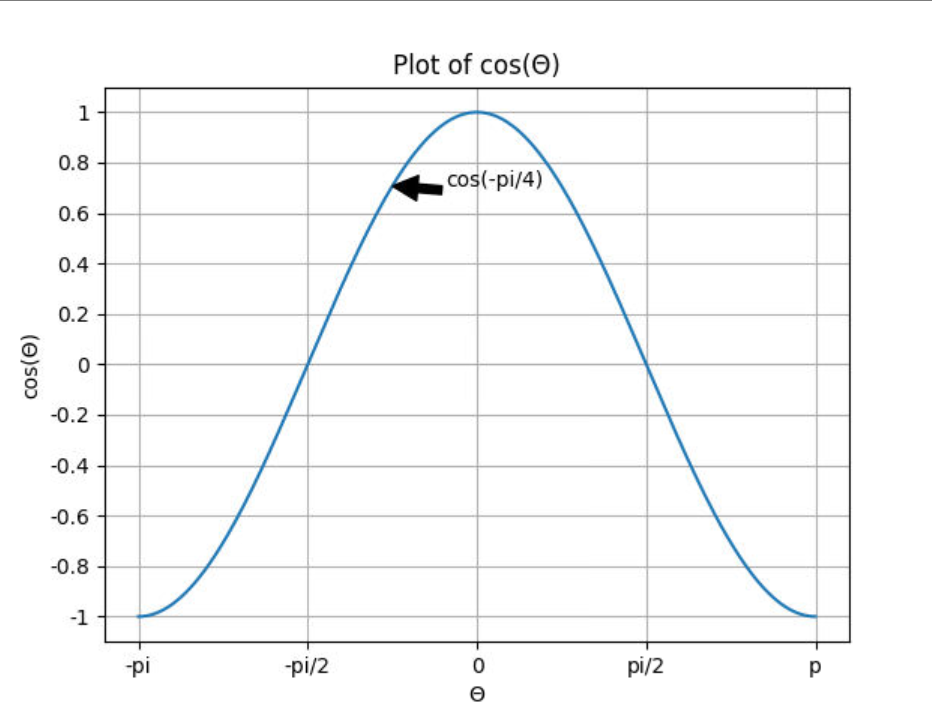
\includegraphics[width=.9\linewidth]{IMAGE.png}\\
[\baselineskip]
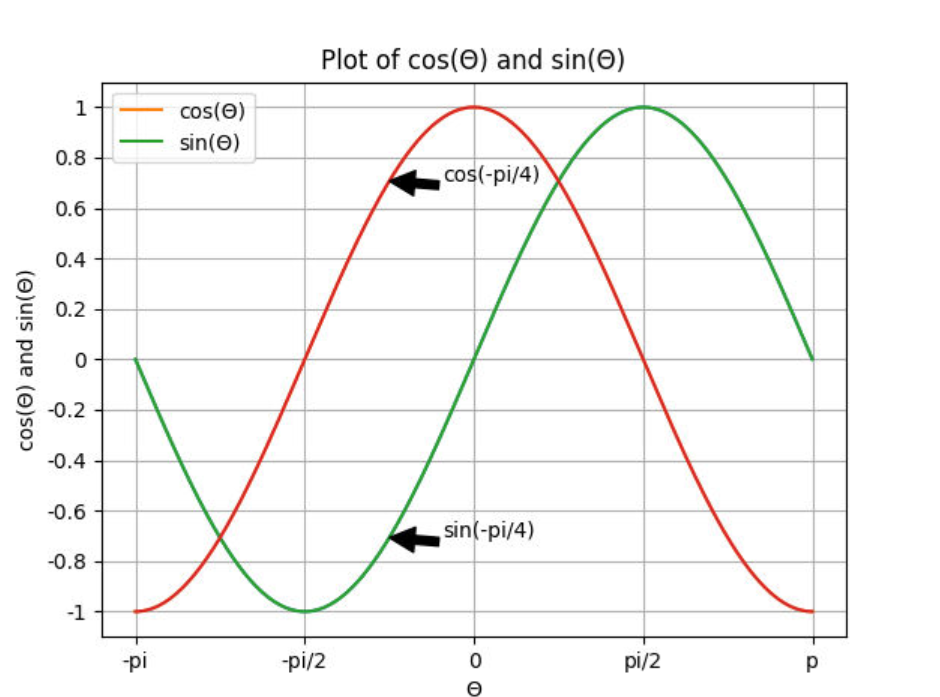
\includegraphics[width=.9
\linewidth]{IMAGE1.png}
\end{center}
%Οι γραφικές παραστάσεις των συναρτήσεων σχεδιάστηκαν χρησιμοποιώντας τη python
\end{document}